\documentclass[12pt]{book}
\usepackage[utf8]{inputenc}
\usepackage[top=1.5cm, bottom=1.5cm, left=1cm, right=1cm]{geometry}
\usepackage{multicol}
\setlength{\columnsep}{1cm}
\usepackage{graphicx}
\usepackage{wrapfig}
\usepackage{wallpaper}
\usepackage[breakable]{tcolorbox}
\graphicspath{{images/}} %Setting the graphicspath

\newtcolorbox{mytextbox}[1][]{%
	standard jigsaw,
	colframe=red,
	opacityframe=0, 
	opacityback=0.7,
	breakable
}

\begin{document}

		\newpage
  \ThisCenterWallPaper{1.2}{80402641a36d31a3ebf2db68f3d6306a}
  \chapter{Kochen}
\begin{mytextbox}
\end{mytextbox}
\newpage
  \chapter{Suppen}
  \ThisCenterWallPaper{1.2}{80402641a36d31a3ebf2db68f3d6306a}
\begin{mytextbox}
\end{mytextbox}
\newpage
	\begin{multicols}{2}
\begin{mytextbox}
  \ThisCenterWallPaper{1.2}{8d3eb2e33142426fff48e29184626861}
  \section{Paprika-Sahne-Hähnchen}



  \begin{center}
    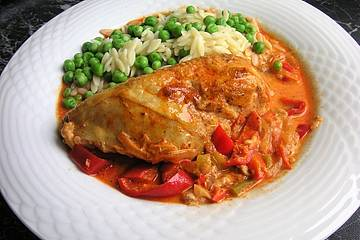
\includegraphics[width=7cm]{8d3eb2e33142426fff48e29184626861}
  \end{center}


  \begin{center}
    Paprika-Sahne-Hähnchen
  \end{center}

  Die Hähnchenfilets waschen und mit Küchenkrepp trocken tupfen. Mit Salz und Paprikapulver würzen und in einer Auflaufform dicht aneinanderlegen. Die Paprikaschoten waschen, entkernen, in schmale Streifen schneiden und auf den Filets verteilen.</br>Die Zwiebel in halbe Ringe schneiden und in einer Pfanne in etwas Öl andünsten. Die Chilischote hineinzupfen, den Knoblauch pressen und hinzugeben. Paprikapulver und Tomatenmark hinzufügen, mit der Brühe ablöschen und kurz aufkochen lassen. Anschließend Sahne und Schmand unter die Soße rühren und mit Salz abschmecken. Die Soße in die Auflaufform gießen, Fleisch und Paprikastreifen sollten ganz bedeckt sein. Den geriebenen Käse gleichmäßig darauf verteilen.</br>Im vorgeheizten Backofen bei 180 °C Ober-/Unterhitze ca. 1/2 Std. garen.</br>Beilagen: Bandnudeln oder Reis und Eisbergsalat mit Mandarinen und süß-saurer Vinaigrette.

\end{mytextbox}\begin{mytextbox}
  \ThisCenterWallPaper{1.2}{8d3eb2e33142426fff48e29184626861}
  \section{Paprika-Sahne-Hähnchen}



  \begin{center}
    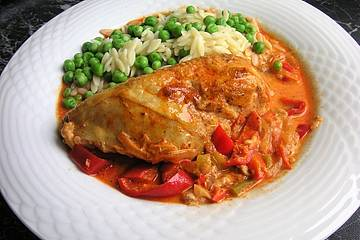
\includegraphics[width=7cm]{8d3eb2e33142426fff48e29184626861}
  \end{center}


  \begin{center}
    Paprika-Sahne-Hähnchen
  \end{center}

  Die Hähnchenfilets waschen und mit Küchenkrepp trocken tupfen. Mit Salz und Paprikapulver würzen und in einer Auflaufform dicht aneinanderlegen. Die Paprikaschoten waschen, entkernen, in schmale Streifen schneiden und auf den Filets verteilen.</br>Die Zwiebel in halbe Ringe schneiden und in einer Pfanne in etwas Öl andünsten. Die Chilischote hineinzupfen, den Knoblauch pressen und hinzugeben. Paprikapulver und Tomatenmark hinzufügen, mit der Brühe ablöschen und kurz aufkochen lassen. Anschließend Sahne und Schmand unter die Soße rühren und mit Salz abschmecken. Die Soße in die Auflaufform gießen, Fleisch und Paprikastreifen sollten ganz bedeckt sein. Den geriebenen Käse gleichmäßig darauf verteilen.</br>Im vorgeheizten Backofen bei 180 °C Ober-/Unterhitze ca. 1/2 Std. garen.</br>Beilagen: Bandnudeln oder Reis und Eisbergsalat mit Mandarinen und süß-saurer Vinaigrette.

\end{mytextbox}	\end{multicols}
  \chapter{Eintöpfe}
  \ThisCenterWallPaper{1.2}{80402641a36d31a3ebf2db68f3d6306a}
\begin{mytextbox}
\end{mytextbox}
\newpage
	\begin{multicols}{2}
\begin{mytextbox}
  \ThisCenterWallPaper{1.2}{8d3eb2e33142426fff48e29184626861}
  \section{Paprika-Sahne-Hähnchen}



  \begin{center}
    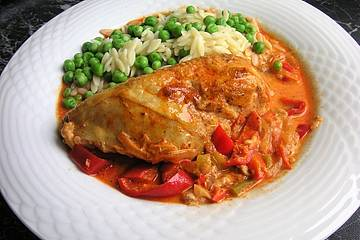
\includegraphics[width=7cm]{8d3eb2e33142426fff48e29184626861}
  \end{center}


  \begin{center}
    Paprika-Sahne-Hähnchen
  \end{center}

  Die Hähnchenfilets waschen und mit Küchenkrepp trocken tupfen. Mit Salz und Paprikapulver würzen und in einer Auflaufform dicht aneinanderlegen. Die Paprikaschoten waschen, entkernen, in schmale Streifen schneiden und auf den Filets verteilen.</br>Die Zwiebel in halbe Ringe schneiden und in einer Pfanne in etwas Öl andünsten. Die Chilischote hineinzupfen, den Knoblauch pressen und hinzugeben. Paprikapulver und Tomatenmark hinzufügen, mit der Brühe ablöschen und kurz aufkochen lassen. Anschließend Sahne und Schmand unter die Soße rühren und mit Salz abschmecken. Die Soße in die Auflaufform gießen, Fleisch und Paprikastreifen sollten ganz bedeckt sein. Den geriebenen Käse gleichmäßig darauf verteilen.</br>Im vorgeheizten Backofen bei 180 °C Ober-/Unterhitze ca. 1/2 Std. garen.</br>Beilagen: Bandnudeln oder Reis und Eisbergsalat mit Mandarinen und süß-saurer Vinaigrette.

\end{mytextbox}	\end{multicols}
  \chapter{Backen}
  \ThisCenterWallPaper{1.2}{80402641a36d31a3ebf2db68f3d6306a}
\begin{mytextbox}
\end{mytextbox}
\newpage
	\begin{multicols}{2}
\begin{mytextbox}
  \ThisCenterWallPaper{1.2}{225e83e76406364e3344e417b312c16b}
  \section{Quinoa Powersalat mit Tomaten und Avocado}



  \begin{center}
    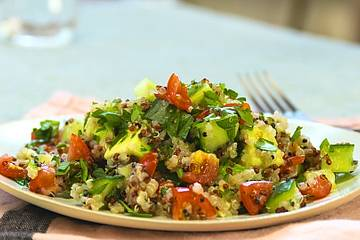
\includegraphics[width=7cm]{225e83e76406364e3344e417b312c16b}
  \end{center}


  \begin{center}
    Quinoa Powersalat mit Tomaten und Avocado
  \end{center}

  Die Quinoa im Sieb waschen, im Topf mit Wasser bedecken, 20 min. kochen. In der Zwischenzeit Tomaten, Avocado und Gurke würfeln, die Petersilie hacken.</br>Die Quinoa sollte dann eine Konsistenz von weichem Reis haben, dann kann man sie unter Wasser abbrausen. Ich stelle das Sieb danach immer auf Küchenkrepp, damit die Quinoa etwas trockener und lockerer wird.</br>Mit den Gemüsewürfeln und der Petersilie vermischen, salzen und nach Geschmack noch etwas pfeffern. Etwas Olivenöl und Chili dazugeben. Aus der Mühle ist Chili ganz besonders frisch und bringt die Verdauung in Schwung. Die leichte Schärfe ist ein guter Gegensatz zur etwas laschen Gurke.</br>Alles schön vermengen und servieren.

\end{mytextbox}\begin{mytextbox}
  \ThisCenterWallPaper{1.2}{8d3eb2e33142426fff48e29184626861}
  \section{Paprika-Sahne-Hähnchen}



  \begin{center}
    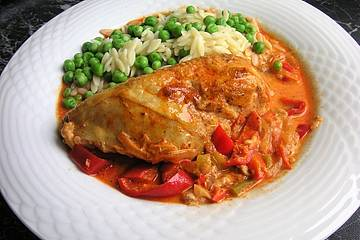
\includegraphics[width=7cm]{8d3eb2e33142426fff48e29184626861}
  \end{center}


  \begin{center}
    Paprika-Sahne-Hähnchen
  \end{center}

  Die Hähnchenfilets waschen und mit Küchenkrepp trocken tupfen. Mit Salz und Paprikapulver würzen und in einer Auflaufform dicht aneinanderlegen. Die Paprikaschoten waschen, entkernen, in schmale Streifen schneiden und auf den Filets verteilen.</br>Die Zwiebel in halbe Ringe schneiden und in einer Pfanne in etwas Öl andünsten. Die Chilischote hineinzupfen, den Knoblauch pressen und hinzugeben. Paprikapulver und Tomatenmark hinzufügen, mit der Brühe ablöschen und kurz aufkochen lassen. Anschließend Sahne und Schmand unter die Soße rühren und mit Salz abschmecken. Die Soße in die Auflaufform gießen, Fleisch und Paprikastreifen sollten ganz bedeckt sein. Den geriebenen Käse gleichmäßig darauf verteilen.</br>Im vorgeheizten Backofen bei 180 °C Ober-/Unterhitze ca. 1/2 Std. garen.</br>Beilagen: Bandnudeln oder Reis und Eisbergsalat mit Mandarinen und süß-saurer Vinaigrette.

\end{mytextbox}	\end{multicols}
\newpage
  \ThisCenterWallPaper{1.2}{80402641a36d31a3ebf2db68f3d6306a}
  \chapter{Trinken}
\begin{mytextbox}
\end{mytextbox}
\newpage


\end{document}